\newpage

\begin{appendices} \addtocontents{toc}{\cftpagenumbersoff{section}}

    \section{Schematics} \label{appendix:schematics}

        \begin{figure}[ht]
            \begin{center}
                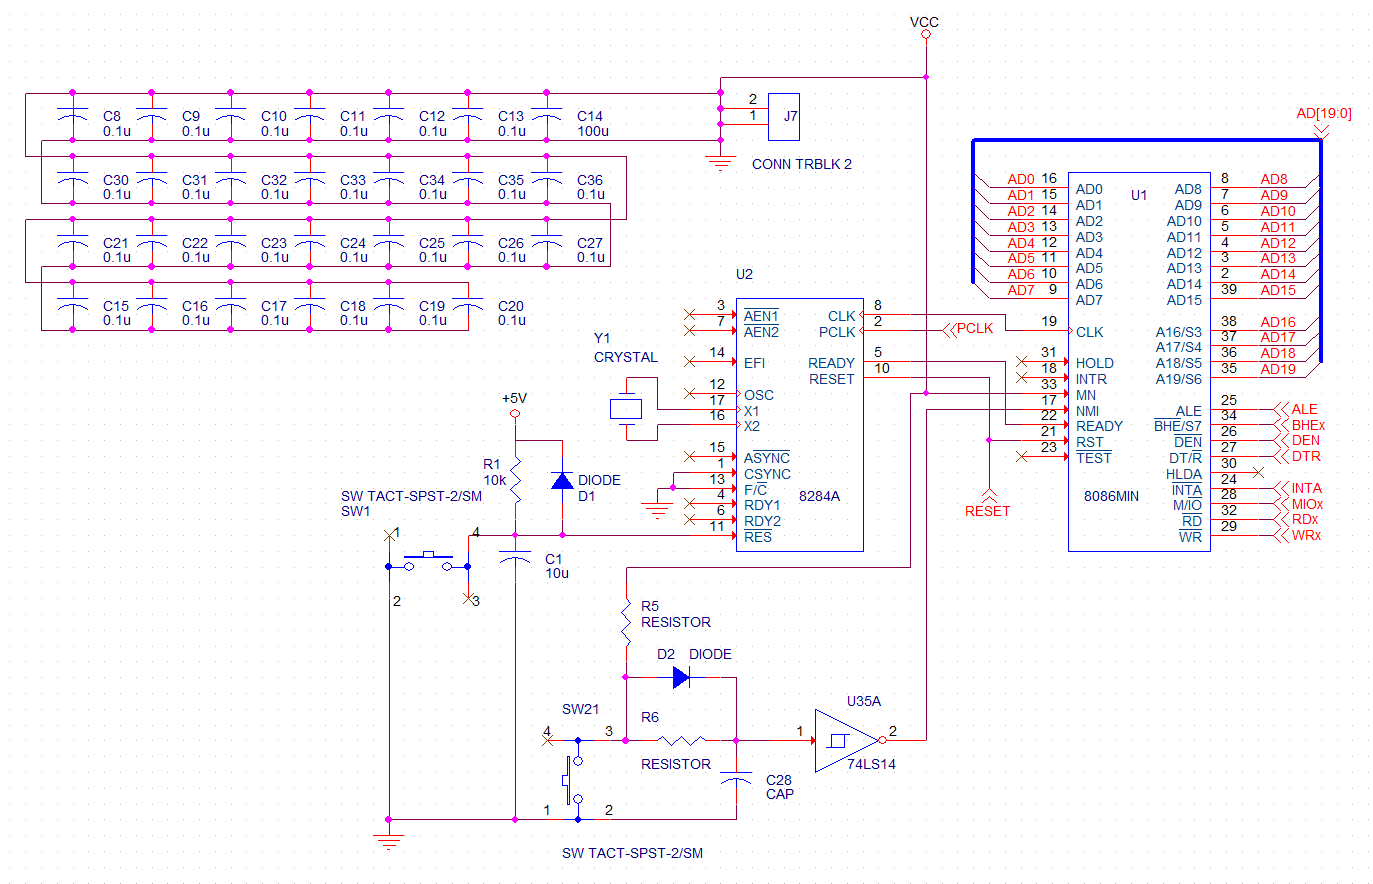
\includegraphics[width=1\textwidth]{figures/schematics/8086.png}
                \caption{8086 Interfaced with the 8284A Clock Generator and its Reset RC Push Button Circuit, and the Power Bank of the Board} \label{fig:page1}
            \end{center}
        \end{figure}

        \begin{figure}[ht]
            \begin{center}
                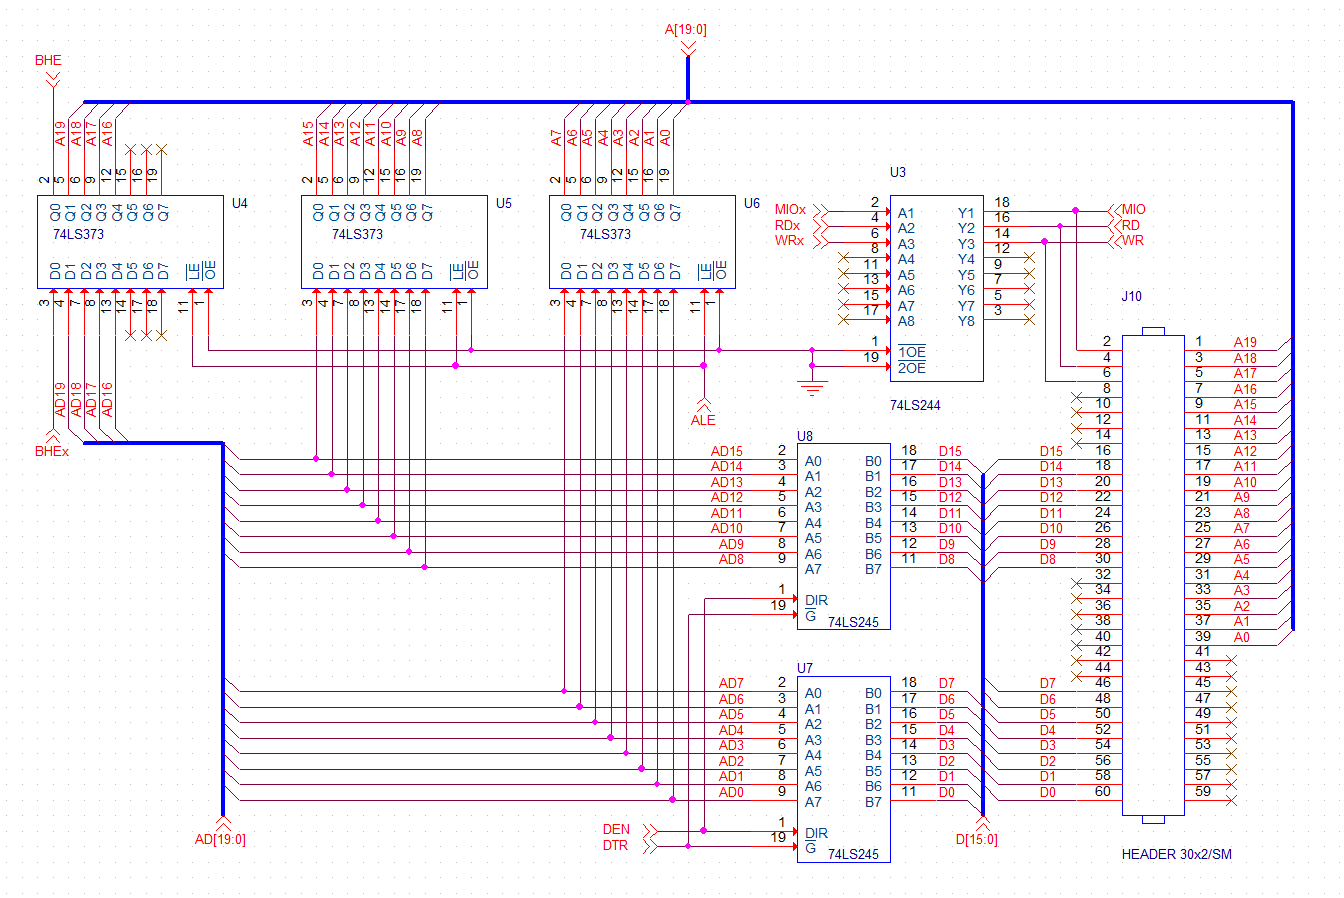
\includegraphics[width=1\textwidth]{figures/schematics/buffers.png}
                \caption{8086 Demultiplexed with Address and Data Buses Pulled into Headers} \label{fig:page2}
            \end{center}
        \end{figure}

        \begin{figure}[ht]
            \begin{center}
                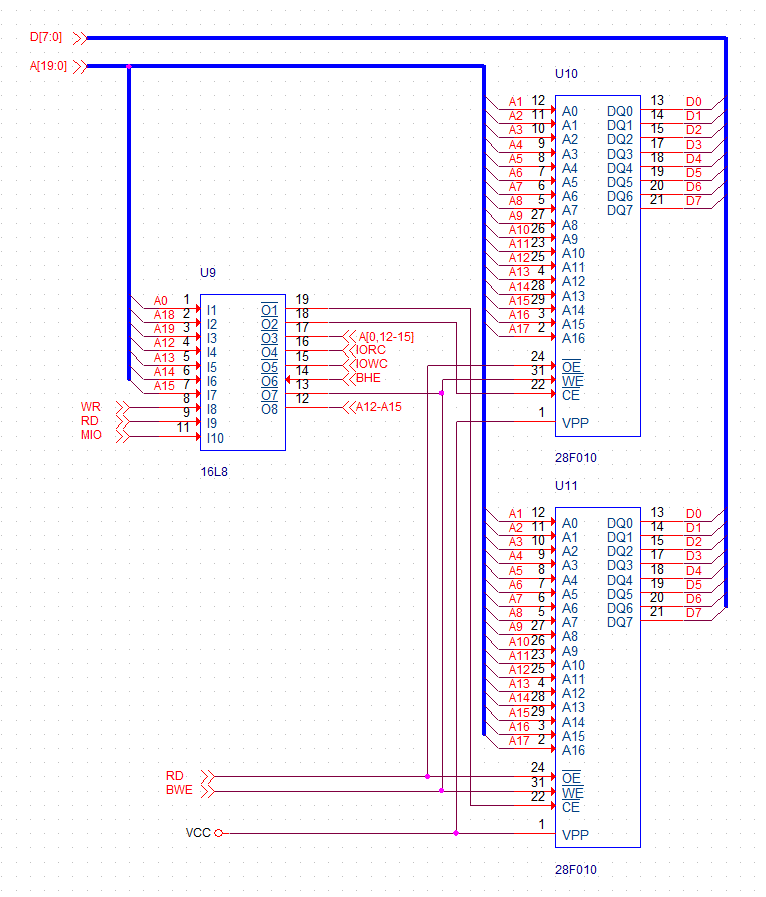
\includegraphics[width=1\textwidth]{figures/schematics/flash_mem.png}
                \caption{256 kB of CMOS Flash Memory and 128 kB Static SRAM} \label{fig:page3}
            \end{center}
        \end{figure}

        \begin{figure}[ht]
            \begin{center}
                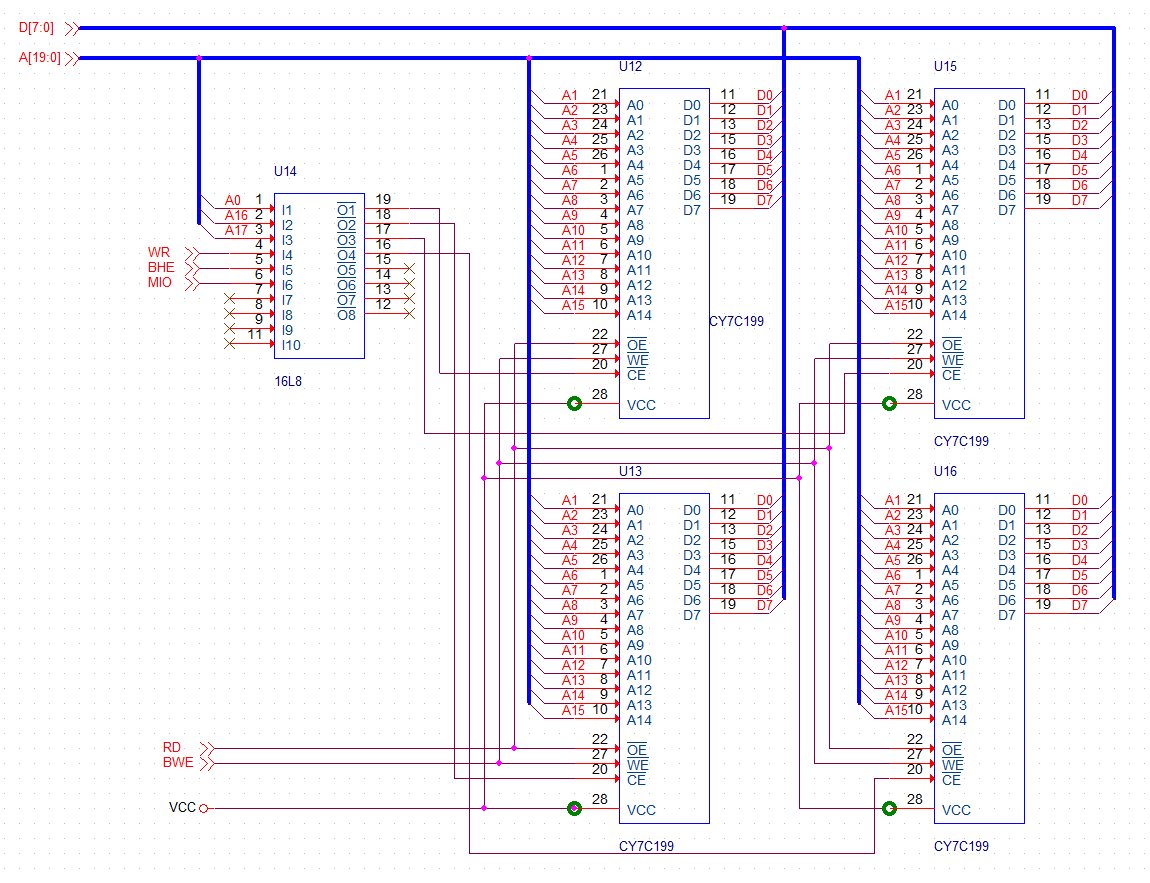
\includegraphics[width=1\textwidth]{figures/schematics/sram.png}
                \caption{128 kB Static SRAM} \label{fig:page4}
            \end{center}
        \end{figure}

        \begin{figure}[ht]
            \begin{center}
                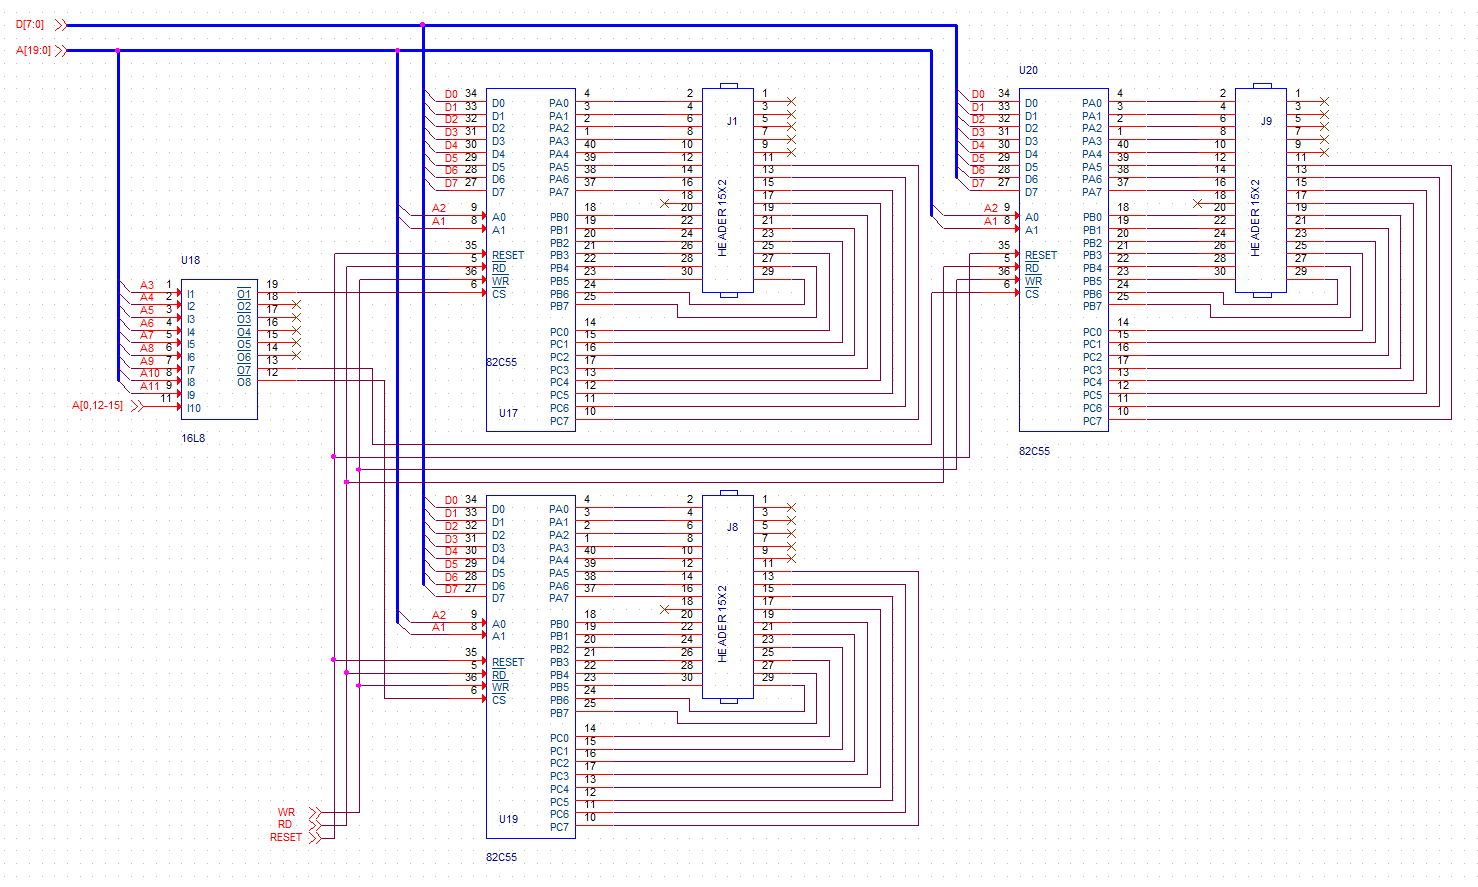
\includegraphics[width=1\textwidth]{figures/schematics/ppi.png}
                \caption{Programmable Peripheral Interface Chips with Port Connections Pulled into Headers} \label{fig:page5}
            \end{center}
        \end{figure}

        \begin{figure}[ht]
            \begin{center}
                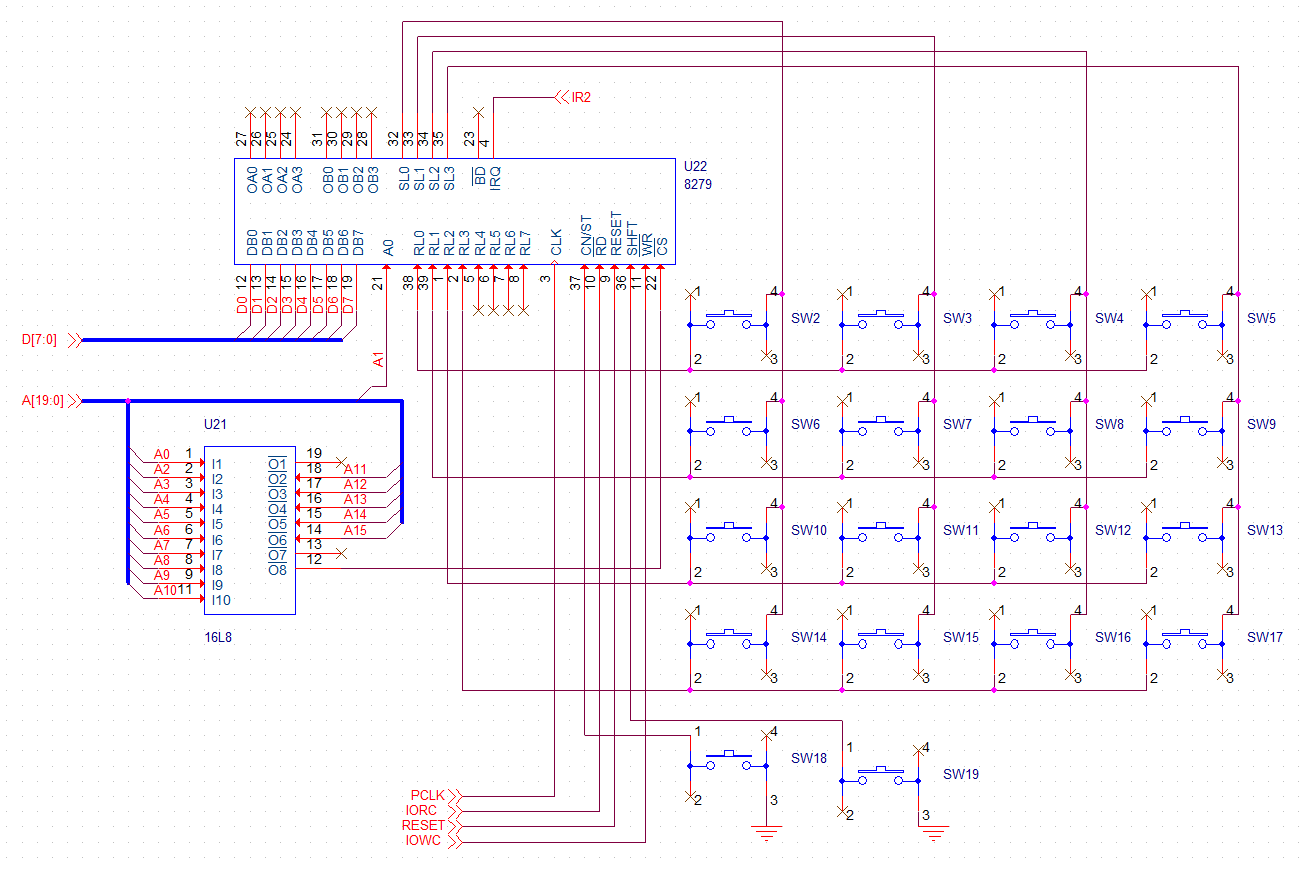
\includegraphics[width=1\textwidth]{figures/schematics/keyboard.png}
                \caption{5$\times$4 Keyboard Matrix} \label{fig:page6}
            \end{center}
        \end{figure}

        \begin{figure}[ht]
            \begin{center}
                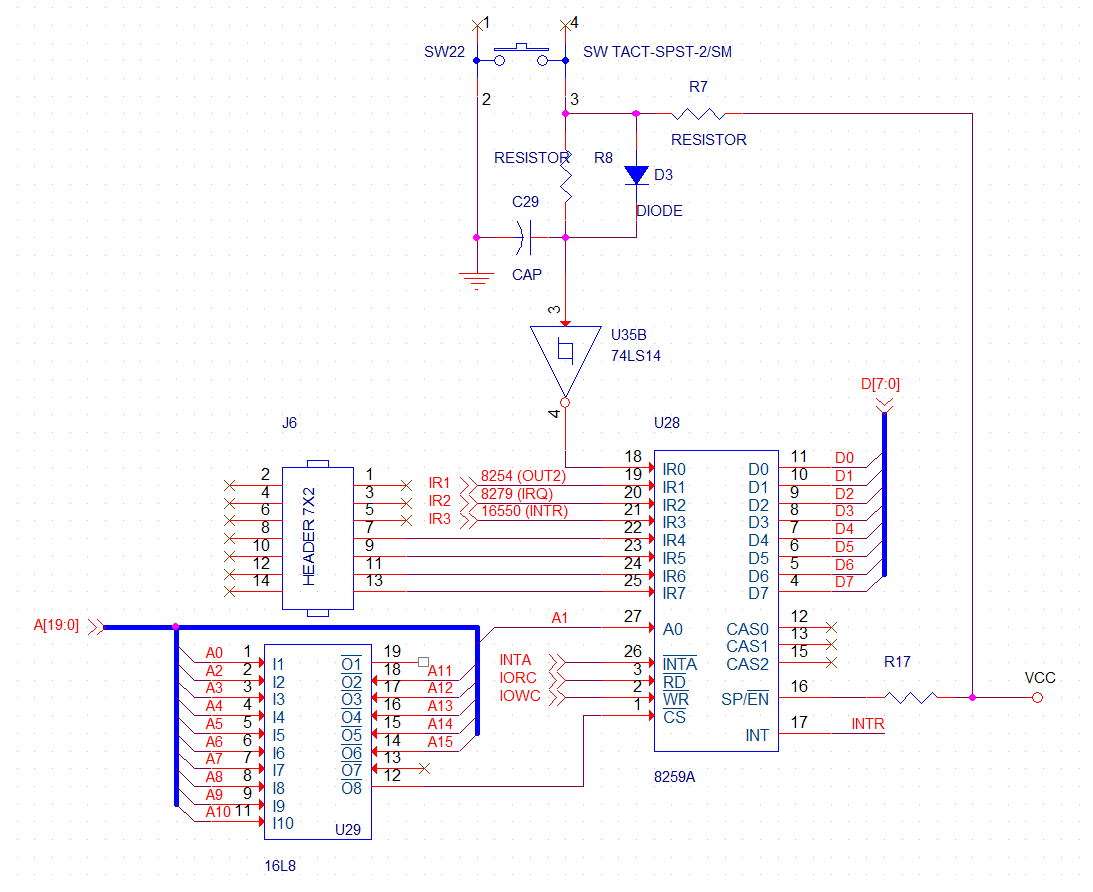
\includegraphics[width=1\textwidth]{figures/schematics/pic.png}
                \caption{Programmable Interval Timer} \label{fig:page7}
            \end{center}
        \end{figure}

        \begin{figure}[ht]
            \begin{center}
                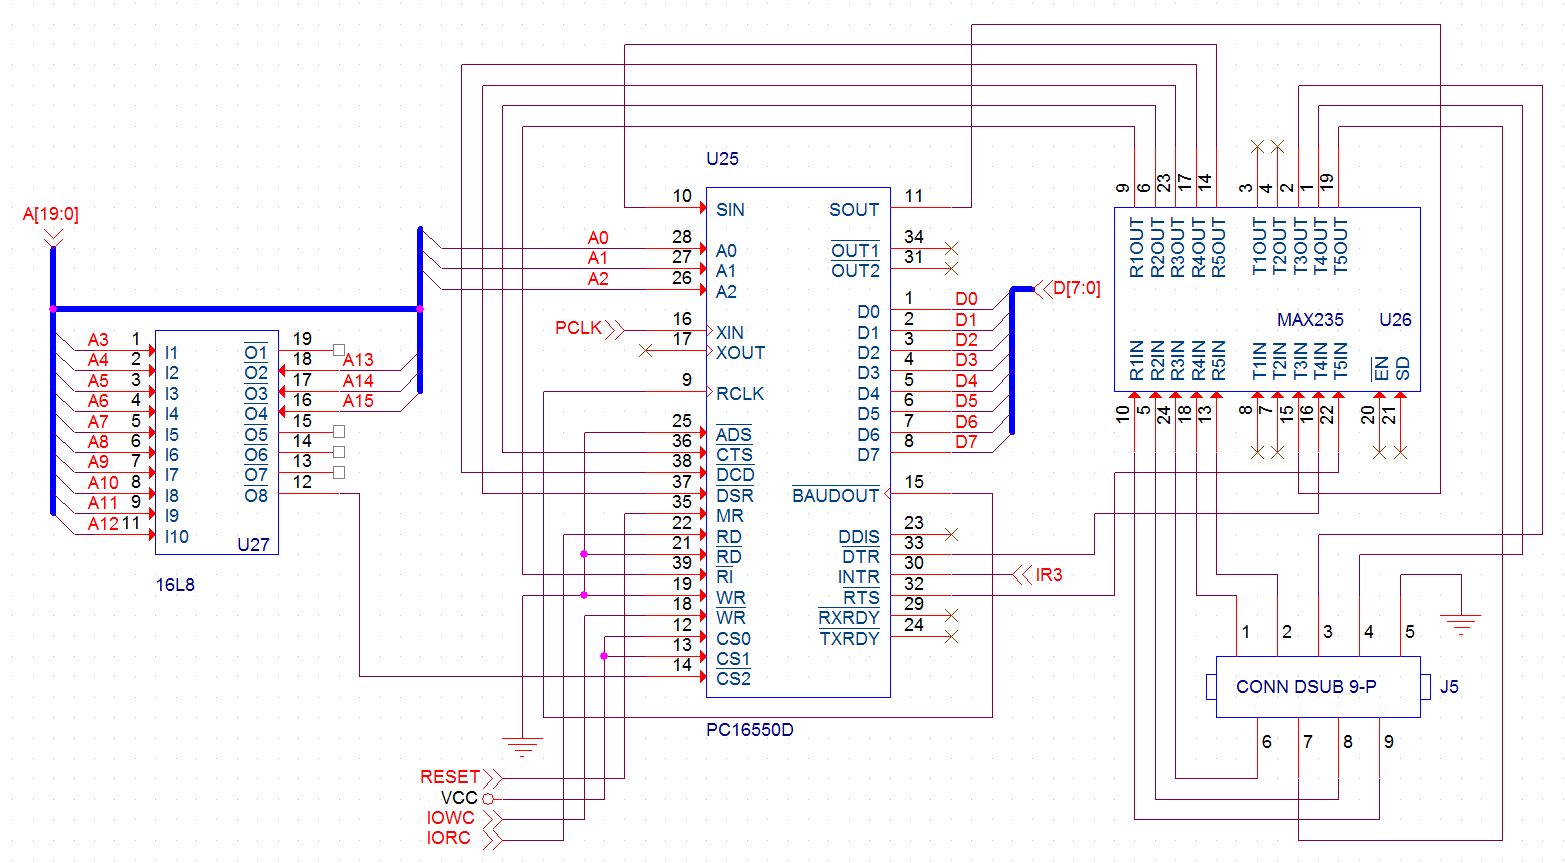
\includegraphics[width=1\textwidth]{figures/schematics/uart.png}
                \caption{UART Connected for Serial Port Using a Line Driver/Receiver and a DSUB-9 connector} \label{fig:page8}
            \end{center}
        \end{figure}

        \begin{figure}[ht]
            \begin{center}
                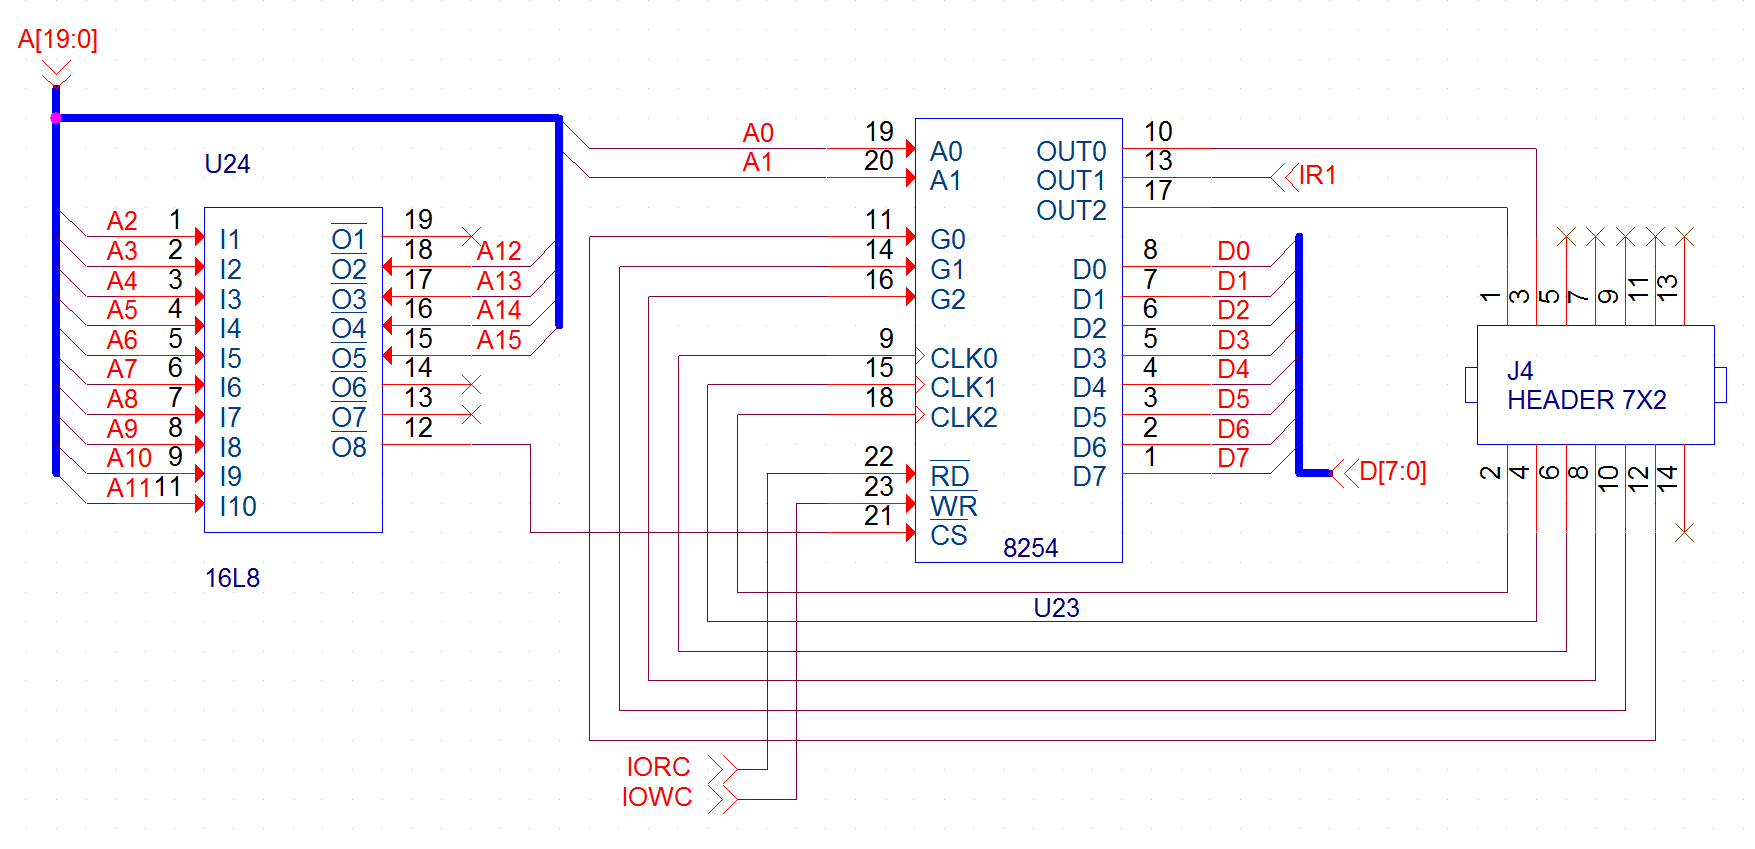
\includegraphics[width=1\textwidth]{figures/schematics/pit.png}
                \caption{Programmable Interrupt Controller with Headers for External Access} \label{fig:page9}
            \end{center}
        \end{figure}

        \begin{figure}[ht]
            \begin{center}
                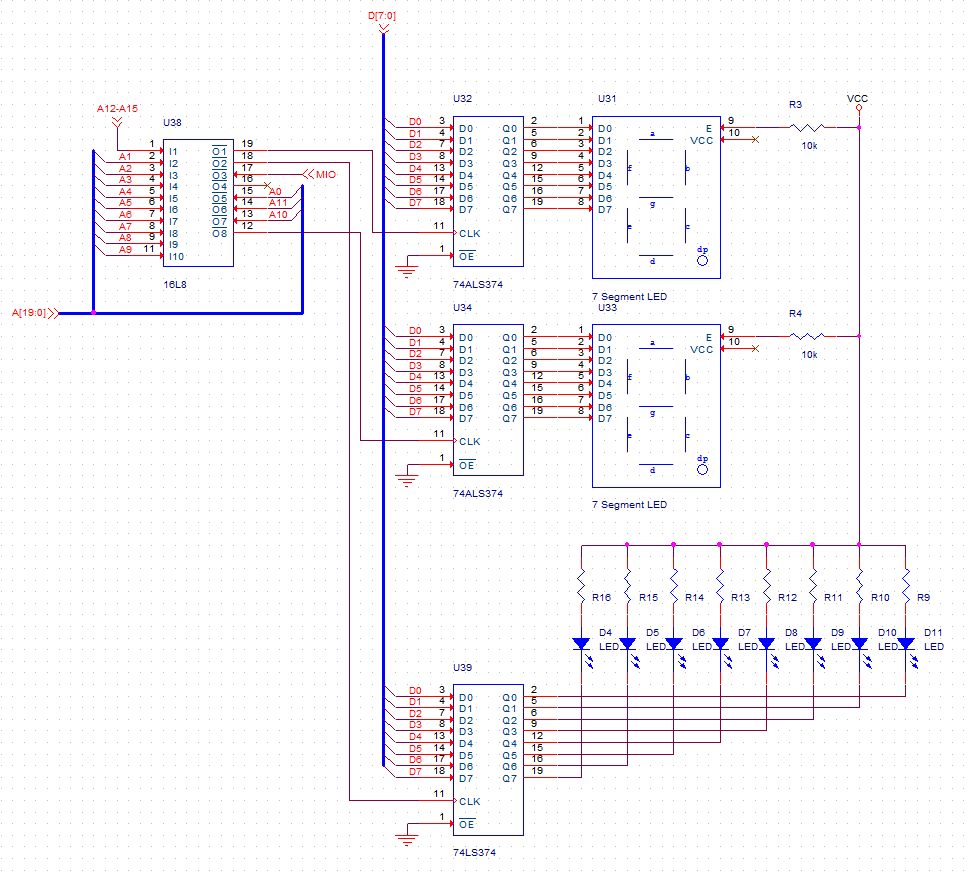
\includegraphics[width=1\textwidth]{figures/schematics/led.png}
                \caption{Common-Anode 7-Segment LEDs with 8 LEDs} \label{fig:page10}
            \end{center}
        \end{figure}

        \begin{figure}[ht]
            \begin{center}
                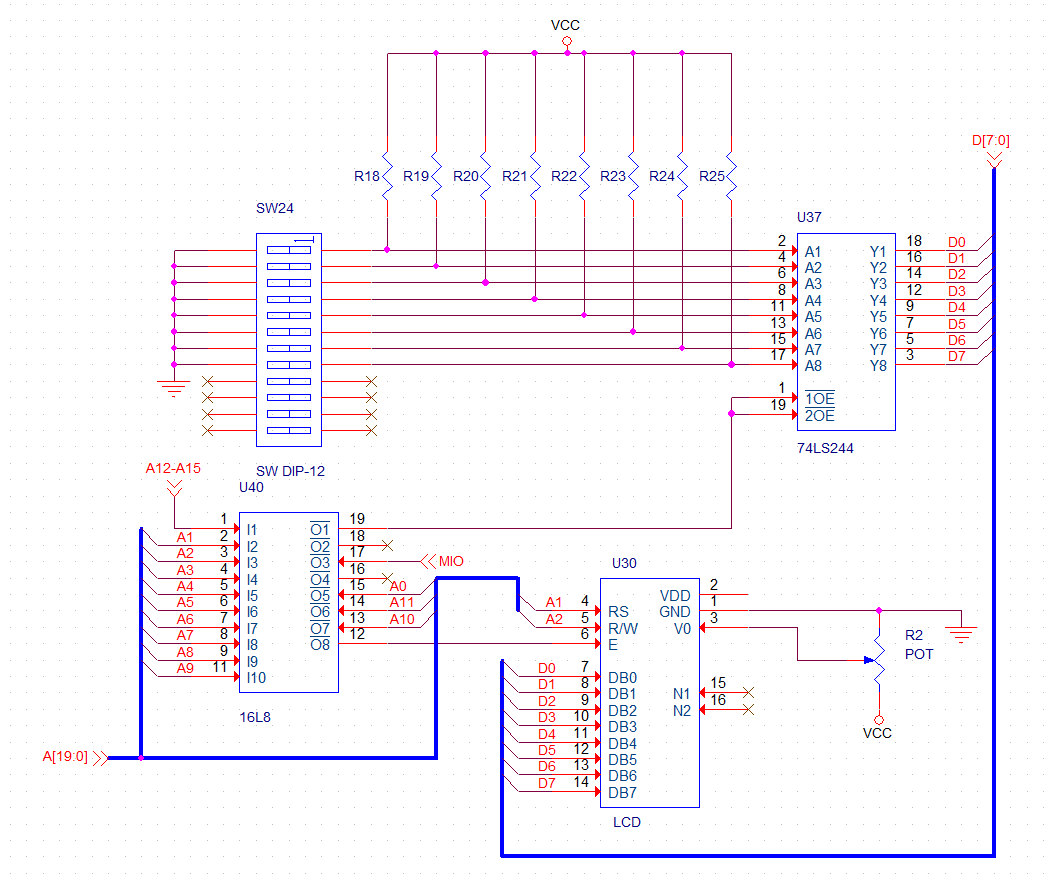
\includegraphics[width=1\textwidth]{figures/schematics/lcd.png}
                \caption{20 character $\times$ 4 line LCD Display with an Integrated LCD Controller} \label{fig:page11}
            \end{center}
        \end{figure}

        \begin{figure}[ht]
            \begin{center}
                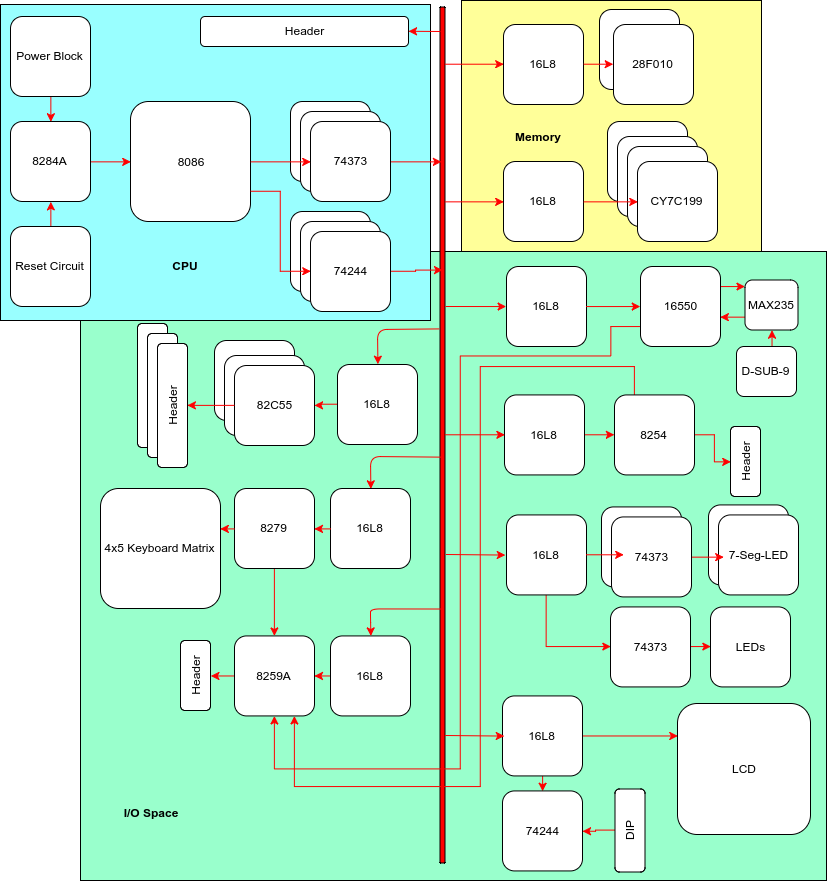
\includegraphics[width=1\textwidth]{figures/block_diagram.png}
                \caption{Overall Block Diagram of all the Schematics of the Board} \label{fig:block_diagram}
            \end{center}
        \end{figure}


    \clearpage
    \newpage

    \section{Code Implementations} \label{appendix:code}

        \subsection{Programmable Logic Devices}

            \subsubsection{U9}

                \VerbatimInput{hdl/u09.vhd}

            \newpage
            \subsubsection{U14}

                \VerbatimInput{hdl/u14.vhd}

            \newpage
            \subsubsection{U18}

                \VerbatimInput{hdl/u18.vhd}

            \newpage
            \subsubsection{U21}

                \VerbatimInput{hdl/u21.vhd}

            \newpage
            \subsubsection{U24}

                \VerbatimInput{hdl/u24.vhd}

            \newpage
            \subsubsection{U27}

                \VerbatimInput{hdl/u27.vhd}

            \newpage
            \subsubsection{U29}

                \VerbatimInput{hdl/u29.vhd}

            \newpage
            \subsubsection{U38}

                \VerbatimInput{hdl/u38.vhd}

            \newpage
            \subsubsection{U40}

                \VerbatimInput{hdl/u40.vhd}

        \newpage
        \subsection{Assembly Implementations}

            \subsubsection{LCD} \label{sec:lcd_asm}
                \VerbatimInput{assembly/lcd.asm}

            \newpage
            \subsubsection{Programmable Peripheral Interface} \label{sec:ppi_asm}
                \VerbatimInput{assembly/ppi.asm}

            \newpage
            \subsubsection{Keyboard} \label{sec:keybrd_asm}
                \VerbatimInput{assembly/keyboard.asm}

            \newpage
            \subsubsection{Programmable Interval Timer} \label{sec:pit_asm}
                \VerbatimInput{assembly/pit.asm}

            \newpage
            \subsubsection{Universal Asynchronous Receiver/Transmitter} \label{sec:uart_asm}
                \VerbatimInput{assembly/uart.asm}


        \clearpage
        \newpage

    \section{PCB Layouts} \label{appendix:pcb}

        \begin{figure}[ht]
            \begin{center}
                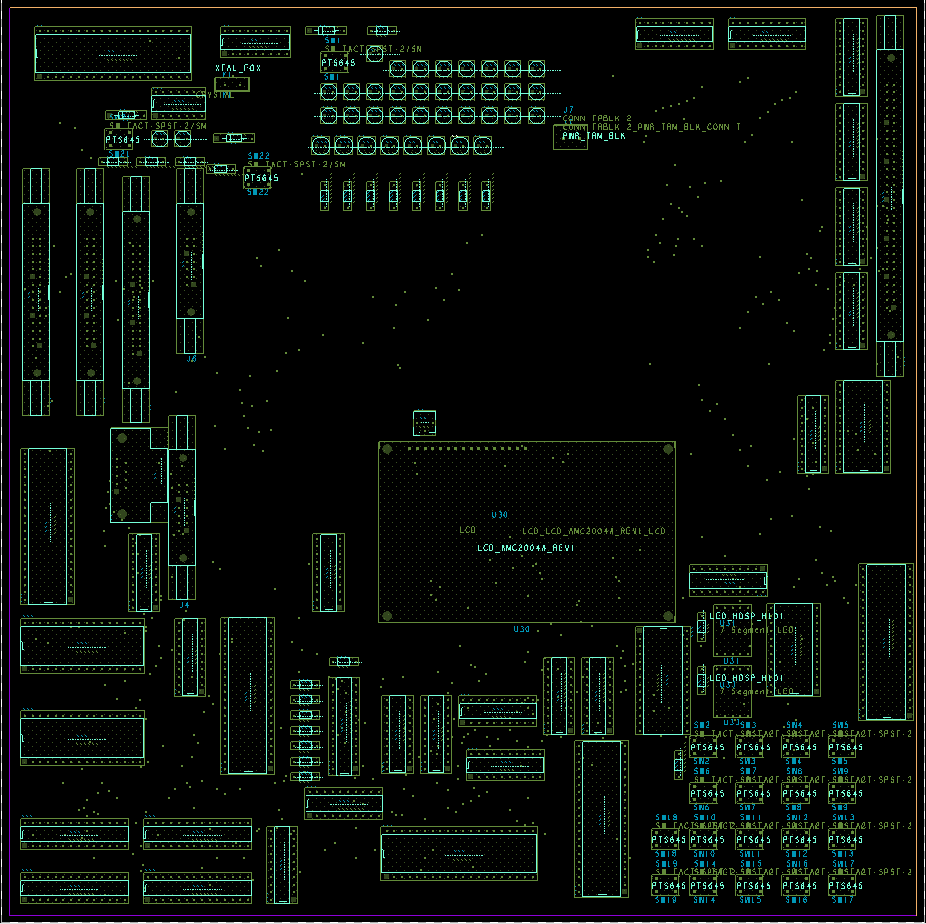
\includegraphics[width=0.9\textwidth]{figures/main.png}
                \caption{Final PCB Layout Showing Only the Components} \label{fig:main}
            \end{center}
        \end{figure}

        \begin{figure}[ht]
            \begin{center}
                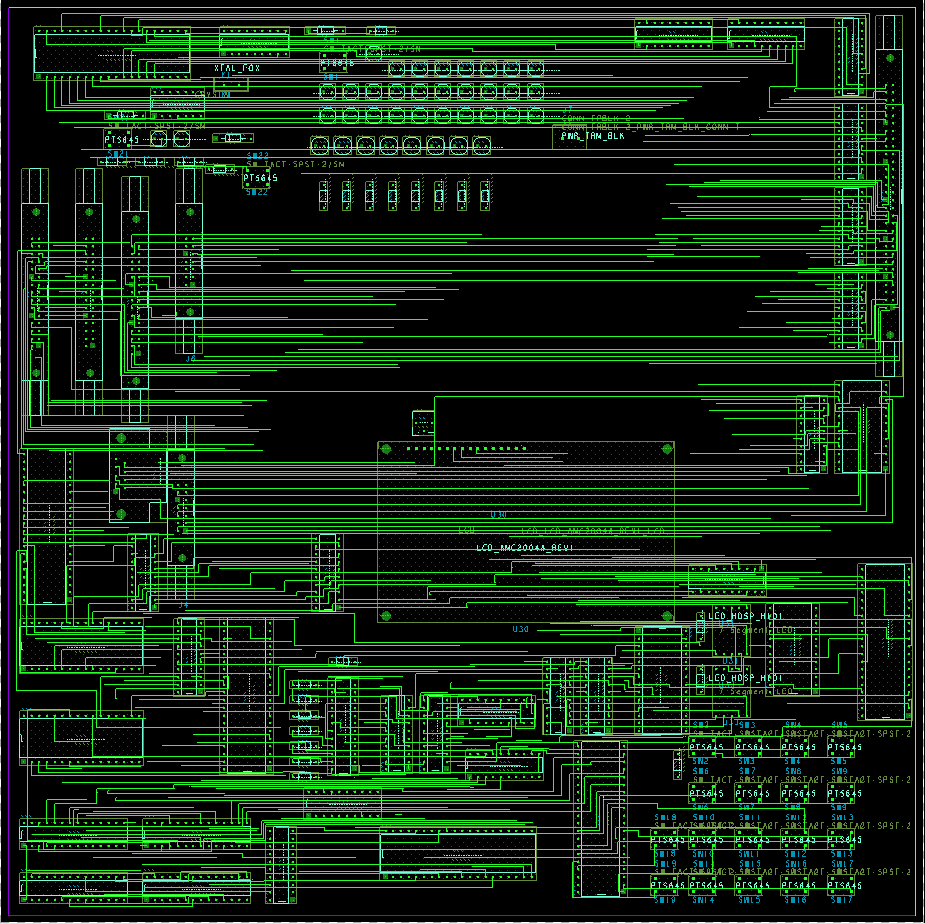
\includegraphics[width=0.95\textwidth]{figures/top.png}
                \caption{Final PCB Layout with only the Top Layer Activated} \label{fig:top}
            \end{center}
        \end{figure}

        \begin{figure}[ht]
            \begin{center}
                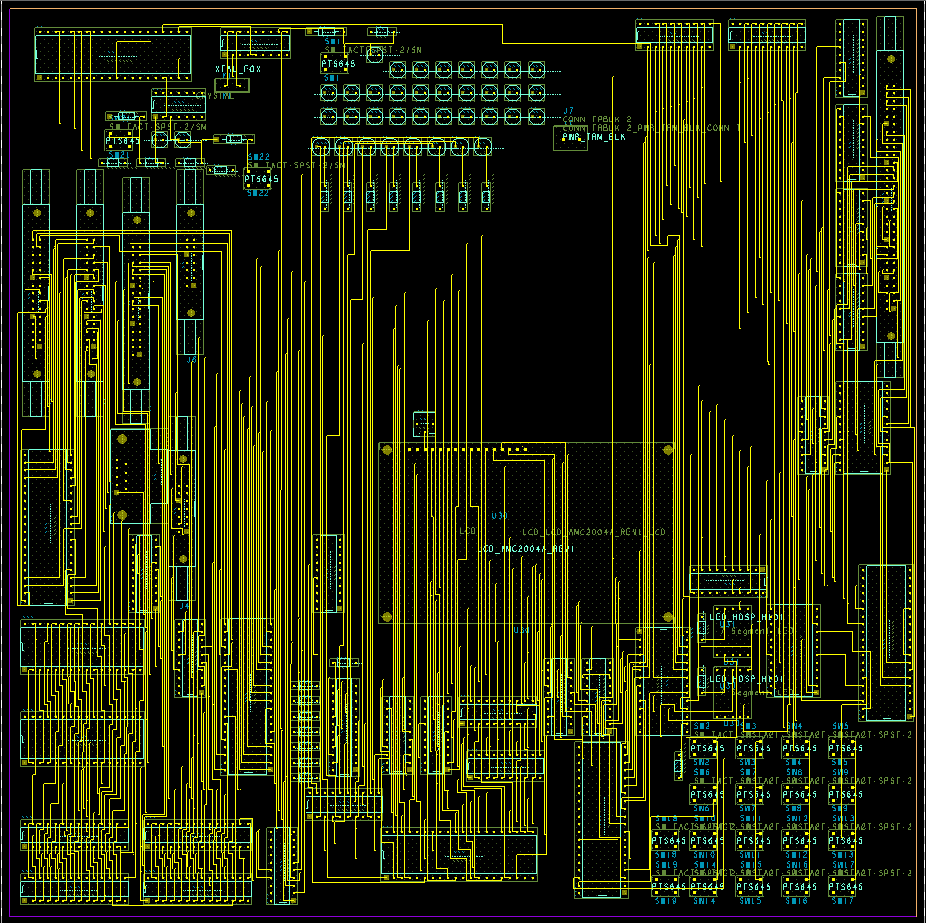
\includegraphics[width=0.95\textwidth]{figures/bottom.png}
                \caption{Final PCB Layout with only the Bottom Layer Activated} \label{fig:bottom}
            \end{center}
        \end{figure}

        \begin{figure}[ht]
            \begin{center}
                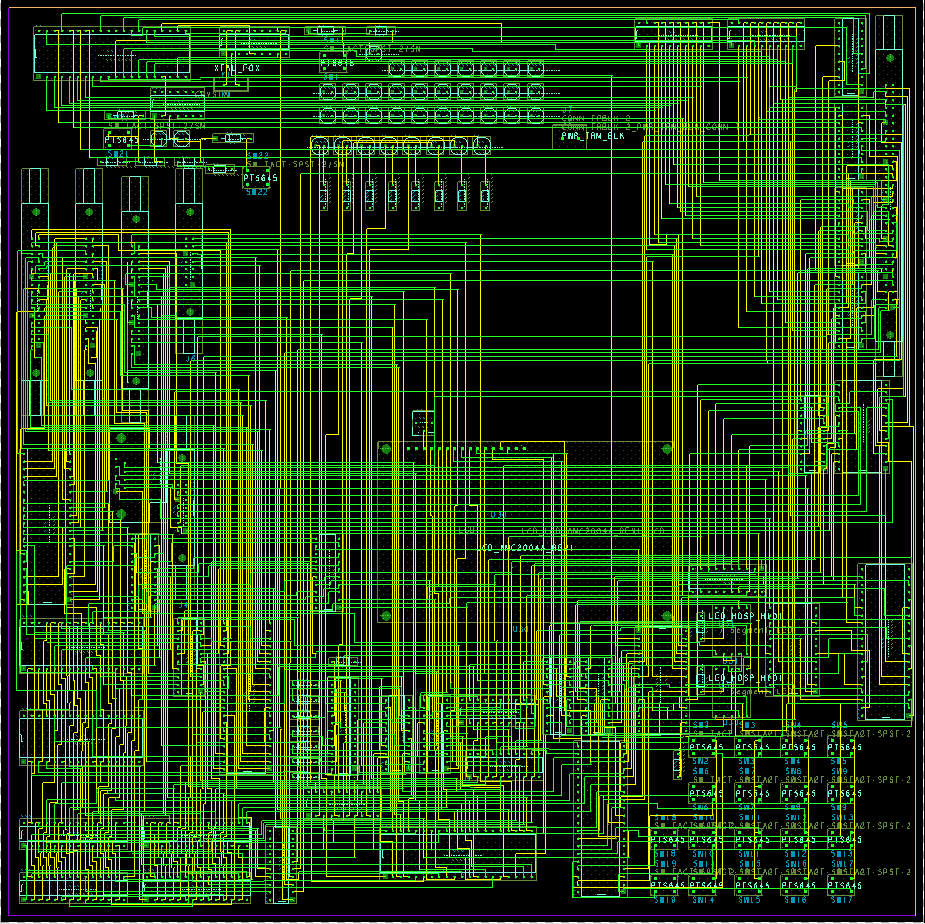
\includegraphics[width=0.95\textwidth]{figures/board.png}
                \caption{Final PCB Layout with all Layers Activated} \label{fig:board}
            \end{center}
        \end{figure}

        \begin{figure}[ht]
            \begin{center}
                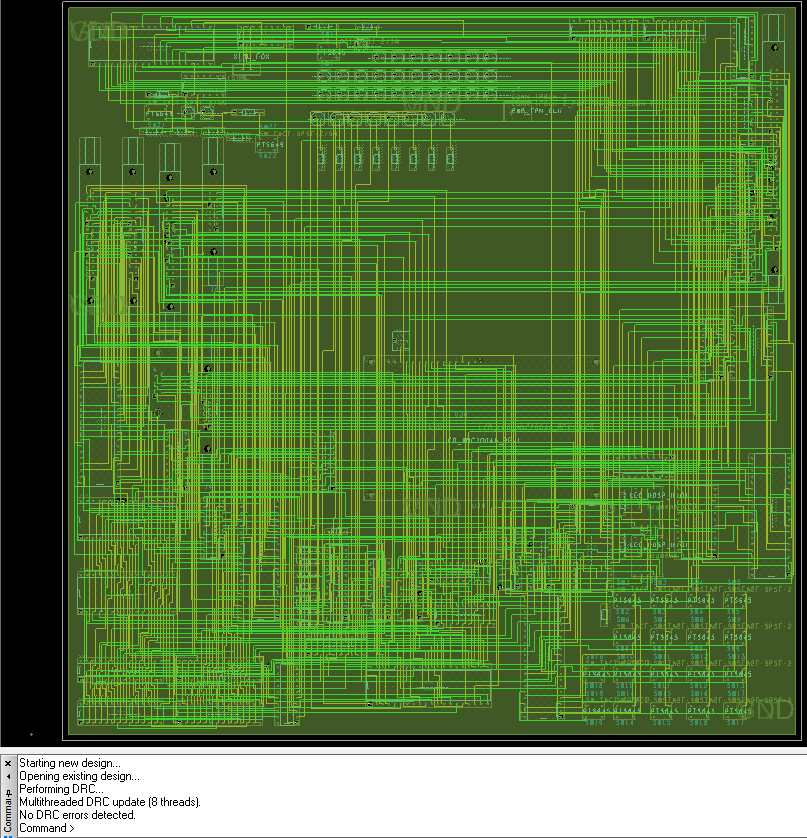
\includegraphics[width=0.95\textwidth]{figures/all.png}
                \caption{Final PCB Layout with all Layers Activated, including Power and Ground} \label{fig:all}
            \end{center}
        \end{figure}

        \clearpage
        \newpage

    \section{Bill of Materials} \label{appendix:bom}

        \def\arraystretch{1.22}
        \begin{table}[H]
            \footnotesize
            \begin{tabular*}{100pt}{@{\extracolsep{\fill}} c p{10cm} p{10cm}}
                \textbf{Amount} & \textbf{Part} & \textbf{Description} \\
                1 & C1 & 10u \\
                26 & C8,C9,C10,C11,C12,C13,C15,C16,\newline
                C17,C18,C19,C20,C21,C22,C23,C24,C25,\newline 
                C26,C27,C30,C31,C32,C33,C34,C35,C36 & 0.1u \\
                1 & C14 & 100u \\
                2 & C28,C29 & CAP \\
                3 & D1,D2,D3 & DIODE \\
                8 & D4,D5,D6,D7,D8,D9,D10,D11 & LED \\
                3 & J1,J8,J9 & HEADER 15X2 \\
                2 & J4,J6 & HEADER 7X2 \\
                1 & J5 & CONN DSUB 9-P \\
                1 & J7 & CONN TRBLK 2 \\
                1 & J10 & HEADER 30x2/SM \\
                11 & R1,R3,R4,R18,R19,R20,R21,R22,\newline
                R23,R24,R25 & 10k \\
                1 & R2 & POT \\
                13 & R5,R6,R7,R8,R9,R10,R11,R12,R13,\newline
                R14,R15,R16,R17 & RESISTOR \\
                3 & SW1,SW21,SW22 & SW TACT-SPST-2/SM \\
                18 & SW2,SW3,SW4,SW5,SW6,SW7,SW8,SW9,\newline
                SW10,SW11,SW12,SW13,SW14,SW15,SW16,SW17,\newline
                SW18,SW19 & SW TACT-SPST-2 \\
                1 & SW24 & SW DIP-12 \\
                1 & U1 & 8086MIN \\
                1 & U2 & 8284A \\
                2 & U3,U37 & 74LS244 \\
                3 & U4,U5,U6 & 74LS373 \\
                2 & U7,U8 & 74LS245 \\
                9 & U9,U14,U18,U21,U24,U27,U29,U38,U40 & 16L8 \\
                2 & U10,U11 & 28F010 \\
                4 & U12,U13,U15,U16 & CY7C199 \\
                3 & U17,U19,U20 & 82C55 \\
                1 & U22 & 8279 \\
                1 & U23 & 8254 \\
                1 & U25 & PC16550D \\
                1 & U26 & MAX235 \\
                1 & U28 & 8259A \\
                1 & U30 & LCD \\
                2 & U31,U33 & 7 Segment LED \\
                2 & U32,U34 & 74ALS374 \\
                1 & U35 & 74LS14 \\
                1 & U39 & 74LS374 \\
                1 & Y1 & CRYSTAL \\
            \end{tabular*}
        \end{table}

        \clearpage

\end{appendices}